% !TeX root = ../thuthesis-example.tex

\chapter{\Project Runtime}\label{chapter-4}

\section{Asynchronous tasks-based inference}
We build \Project on top of FlexFlow~\cite{flexflow,unity}, a distributed DNN framework originally designed for training. We extend FlexFlow to support inference. FlexFlow itself is built on top of Legion~\cite{legion} (Section \ref{legion}), a data-centric parallel programming framework. We reuse FlexFlow's abstractions for deep learning, in particular the Layer, Tensor, ParallelTensor and Operator abstractions. Thanks to these abstractions, we can build the MoE model using a similar API to PyTorch or Tensorflow, and use FlexFlow's compiler to automatically translate it into a parallel computational graph, where each node is an asynchronous task, and each edge is a data dependency. 

\subsection{Legion}\label{legion}
Legion is an asynchronous, task-based distributed execution engine. Tasks are the basic units of the Legion parallel computation, their execution is non-preemptible, and they can call any C++ function, including those allocating/de-allocating memory, but they cannot use packages other than Legion to implement parallelism or concurrency. To write a Legion program, the user implements each task as a C++ function (which may call other functions), and defines each task's input/outputs using Legion logical regions. 

Internally, tasks are defined as operations that transform one or more logical regions, and the system automatically schedules and executes these tasks in parallel, based on their dependencies and resource availability. 

In Legion, control flow is handled using a dynamic dependency graph, which represents the dependencies between different tasks and logical regions. As tasks complete, the system automatically updates the graph and schedules new tasks to execute, based on their dependencies. This approach provides a more flexible and expressive way to manage control flow, and can adapt to changes in the system at runtime.

\subsection{Mapping}
The system provides a programming model that is based on the concept of logical regions, which are abstract data structures that can be mapped to physical memory resources in a way that is transparent to the programmer. The Legion mapping interface is the mechanism through which the logical regions are mapped to physical resources. The interface provides a set of functions that allow the programmer to specify how the logical regions should be mapped, as well as to query the system for information about the mapping. The mapping interface also provides a mechanism for specifying constraints on the mapping. These constraints can be used to specify affinity between the logical region and the physical resources, as well as to specify other properties of the mapping, such as the layout of the physical memory.

Legion allows the programmer to register a custom mapper to make the mapping policy decisions. In \Project we largely reuse the FlexFlow custom mapper, with a few modifications. In particular, we manually map the operators according to the parallelization plan discussed in Section \ref{design-parallelization}.


\section{Debugging and Profiling}
One advantage of building our system on top of Legion is the ability to use all the Legion tools that are available for debugging and profiling. In particular, during the development of \Project we frequently used Legion Spy~\footnote{\url{https://legion.stanford.edu/debugging/index.html\#legion-spy}} as well Legion Prof~\footnote{\url{https://legion.stanford.edu/profiling/\#legion-prof}} for profiling. For instance, a screenshot of the profiling results from our MoE inference application is shown below:
\begin{figure}[H]
    \centering
    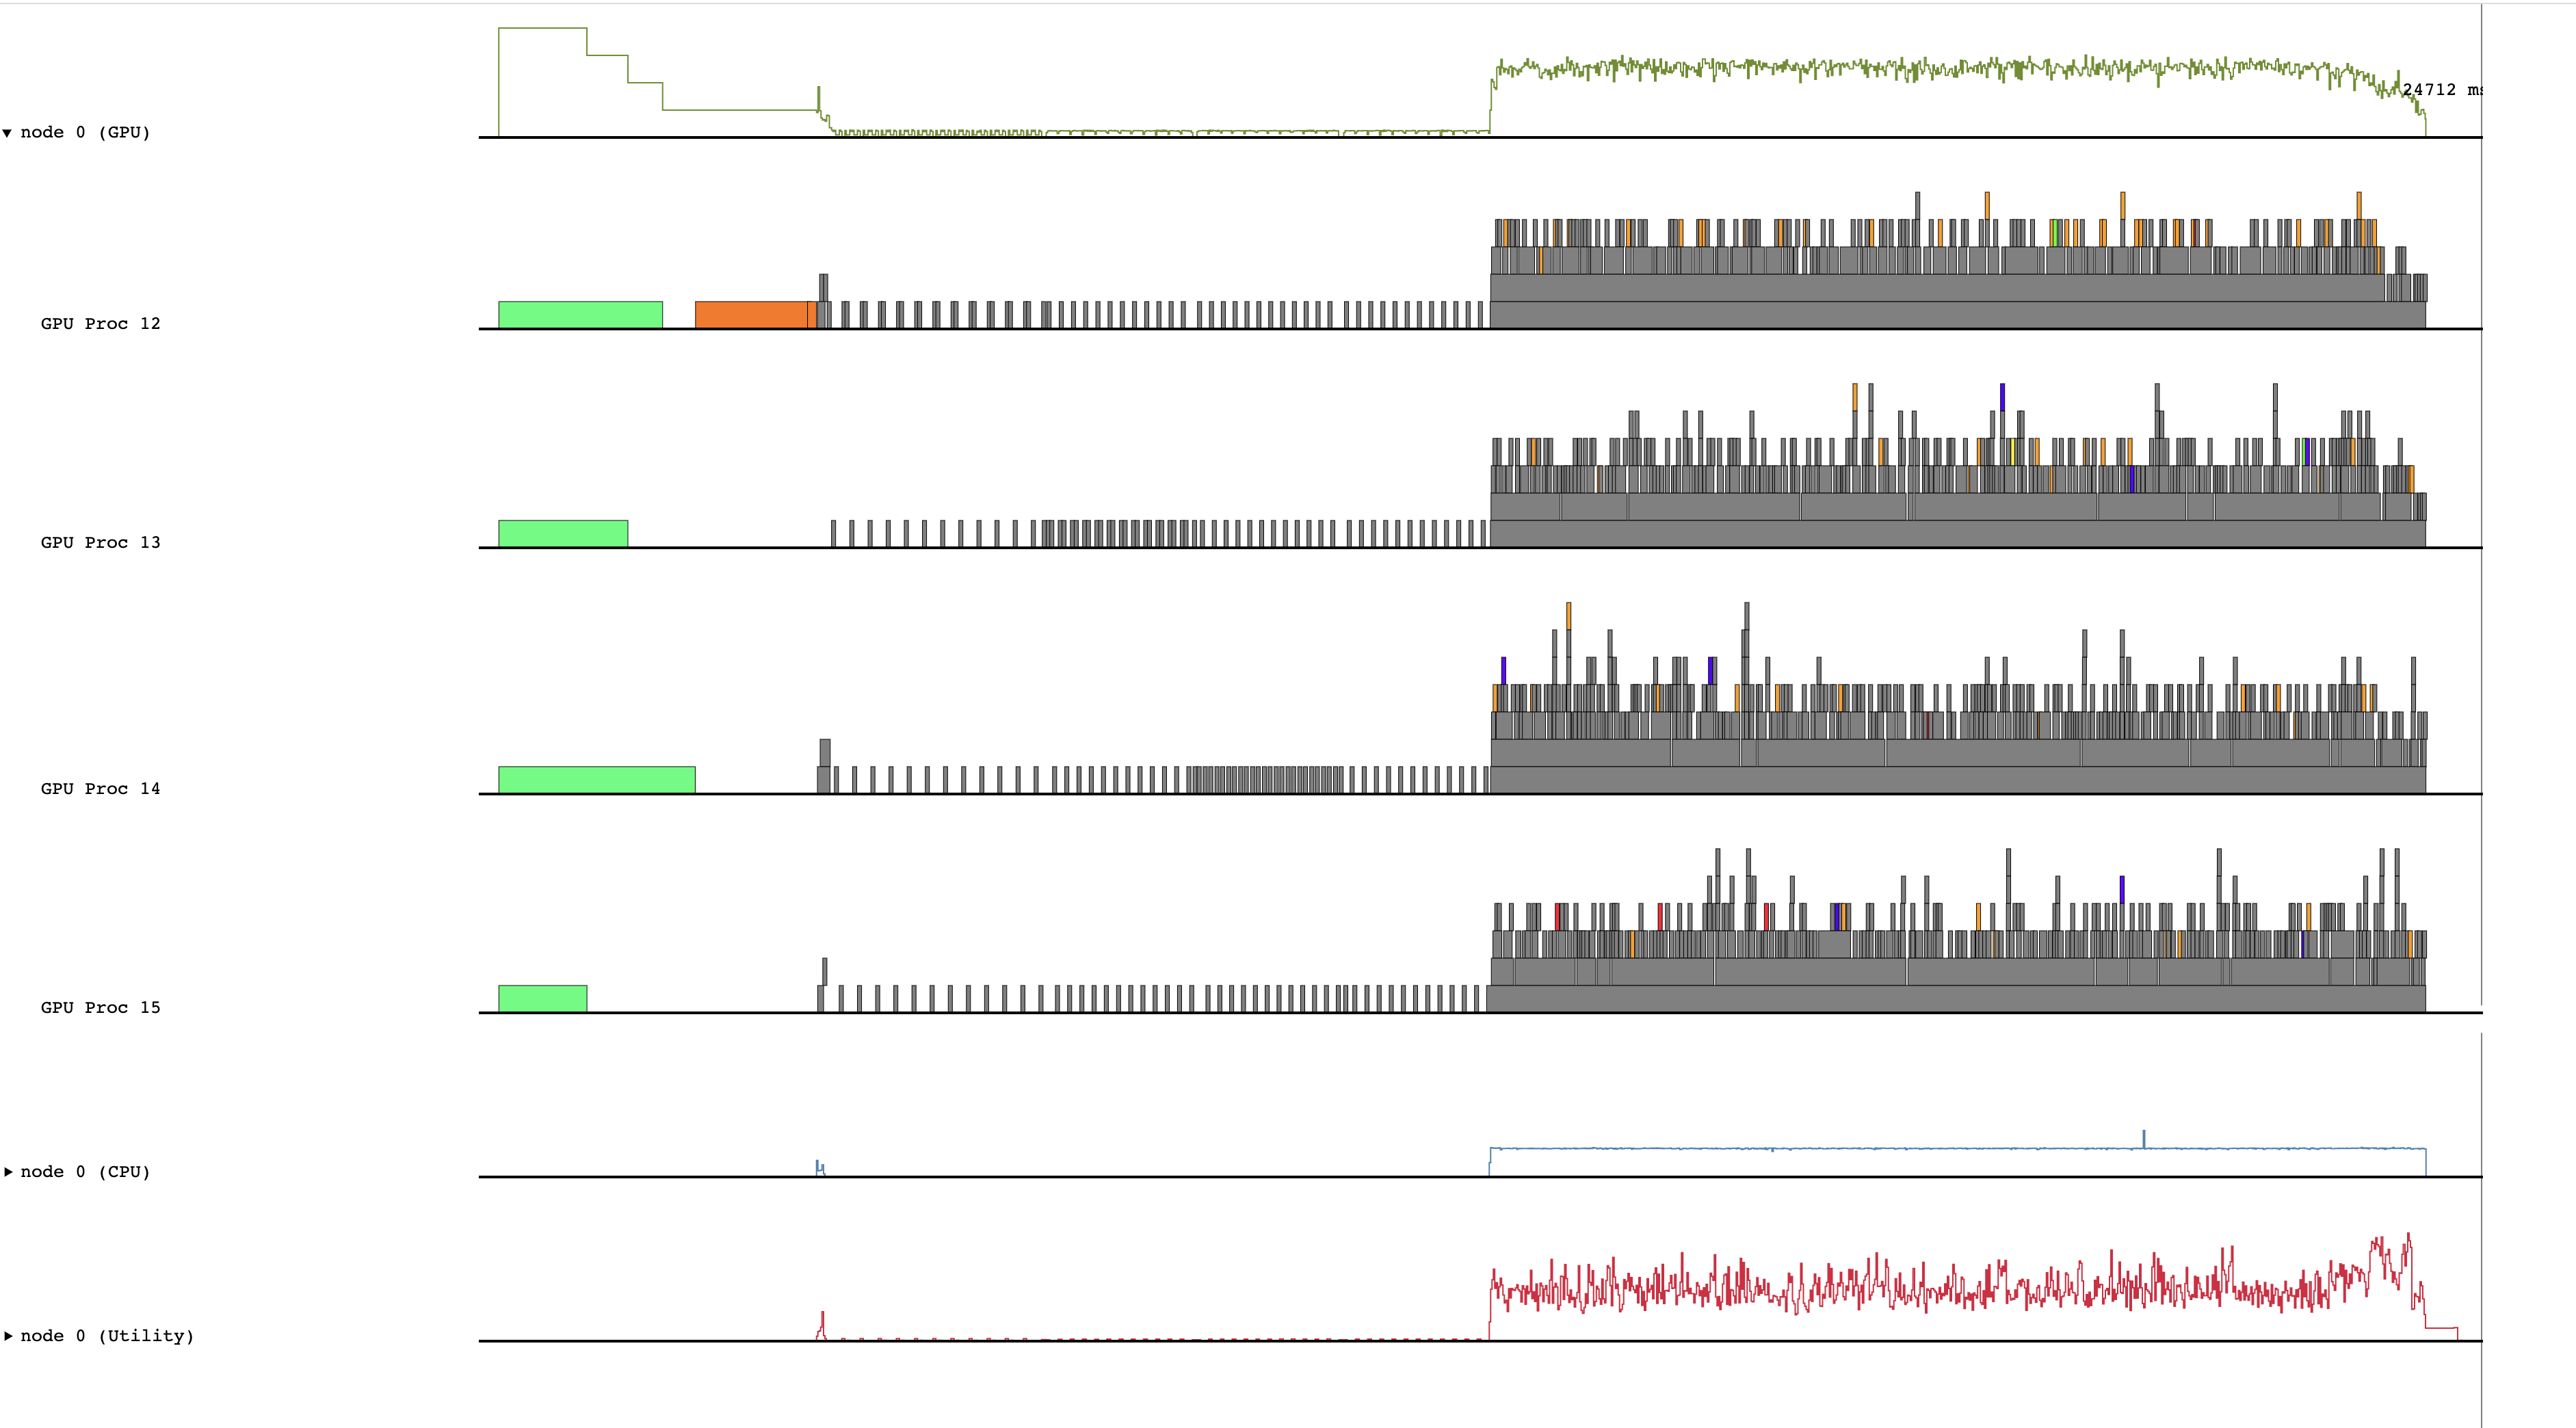
\includegraphics[width=\linewidth]{figures/legion_prof0.png}
    \caption{\textbf{Legion Prof} output for a \Project test run}
    \label{fig:legion-prof0}
\end{figure}
From the figure, we can check the utilization of each CPU and GPU, the communication between nodes, and much more. Zooming in (see for example Figure \ref{fig:legion-prof1}) we can see each task individually, and get more fine-grained details, such as whether a CPU/GPU task is blocking.
\begin{figure}[H]
    \centering
    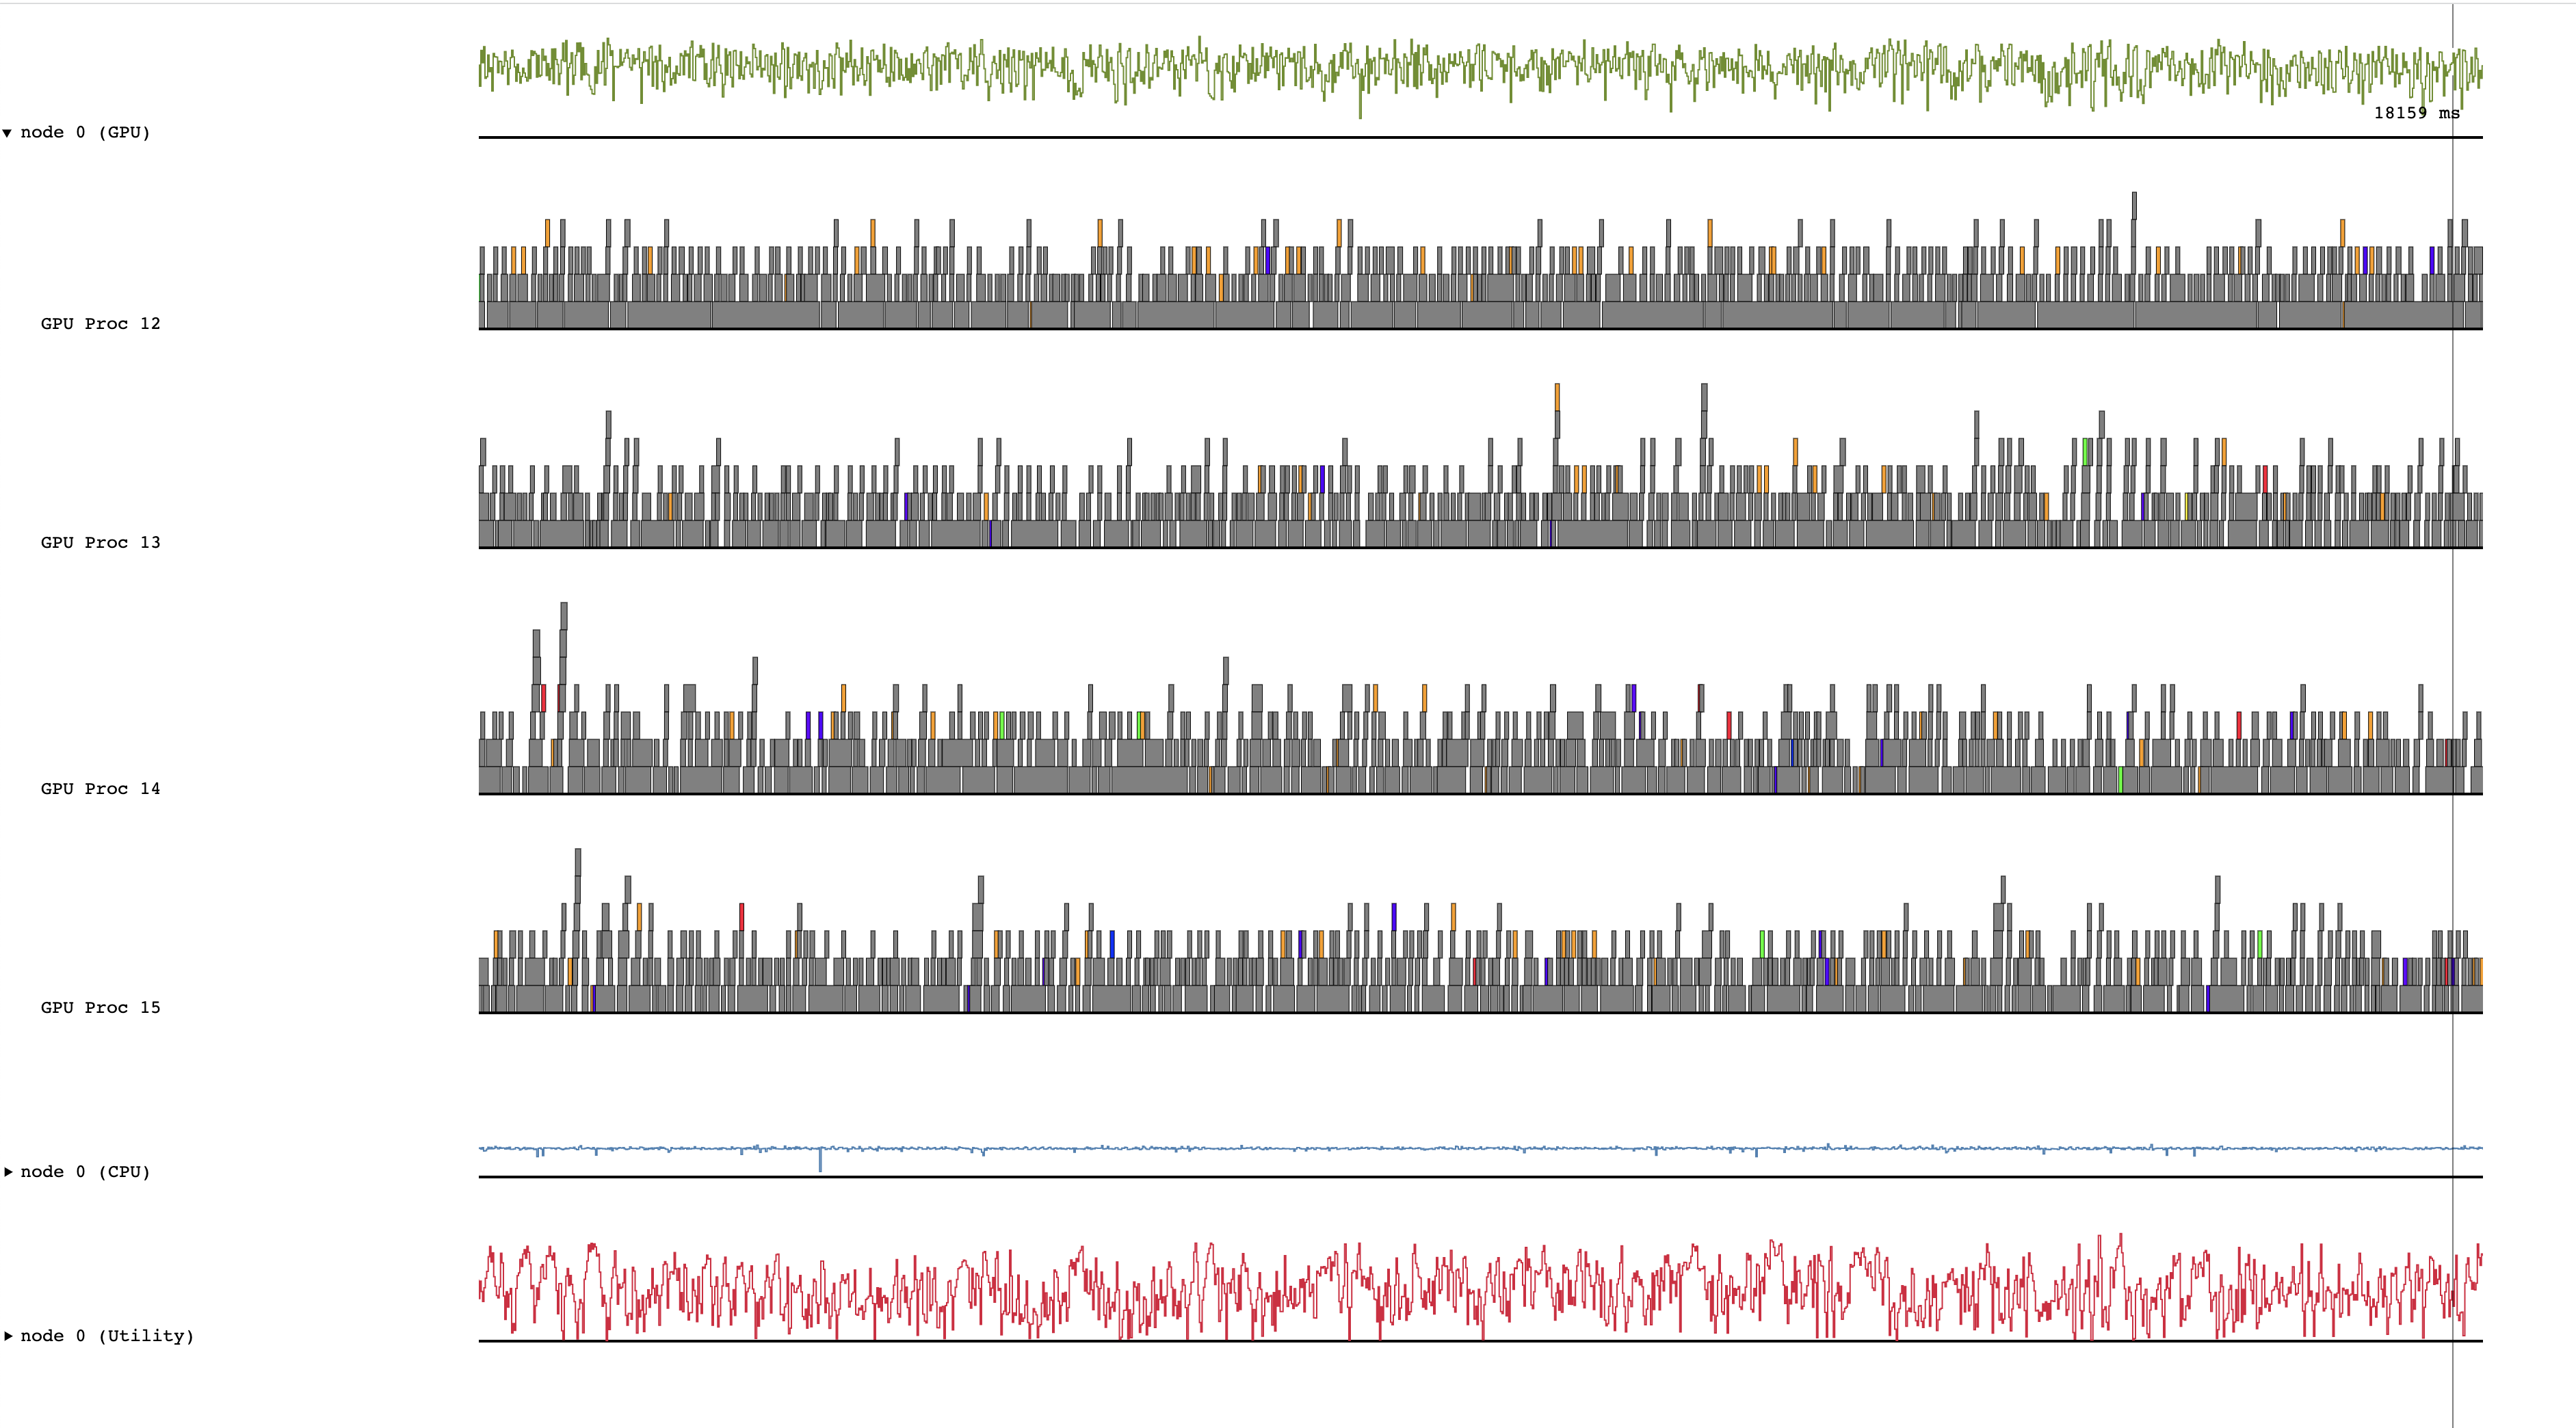
\includegraphics[width=\linewidth]{figures/legion_prof1.png}
    \caption{\textbf{Legion Prof} output for a \Project test run (zoomed in)}
    \label{fig:legion-prof1}
\end{figure}